Калибровка спектрометра была выполнена по спектрам ртути и неона. По ртути
следует калиброваться в коротковолновой части спектра, а по неону -- в средней и
длинноволновой.

\begin{table}[h!]
  \centering
  \caption{Калибровка для неона}
  \begin{tabular}{| c | c | c |}
  \hline
  $\lambda, A$ & $\theta, дел$ & $\sigma_{\theta}, дел$ \\
  \hline
  $7032$       & $2942$        & $5$                    \\
  \hline
  $6929$       & $2914$        & $5$                    \\
  \hline
  $6717$       & $2850$        & $5$                    \\
  \hline
  $6678$       & $2830$        & $5$                    \\
  \hline
  $6599$       & $2804$        & $5$                    \\
  \hline
  $6533$       & $2782$        & $5$                    \\
  \hline
  $6507$       & $2770$        & $5$                    \\
  \hline
  $6402$       & $2735$        & $5$                    \\
  \hline
  $6383$       & $2724$        & $5$                    \\
  \hline
  $6334$       & $2708$        & $5$                    \\
  \hline
  $6305$       & $2696$        & $5$                    \\
  \hline
  $6267$       & $2682$        & $5$                    \\
  \hline
  $6217$       & $2664$        & $5$                    \\
  \hline
  $6164$       & $2638$        & $5$                    \\
  \hline
  $6143$       & $2638$        & $5$                    \\
  \hline
  $6096$       & $2614$        & $5$                    \\
  \hline
  $6074$       & $2602$        & $5$                    \\
  \hline
  $6030$       & $2584$        & $5$                    \\
  \hline
  $5976$       & $2558$        & $5$                    \\
  \hline
  $5945$       & $2548$        & $5$                    \\
  \hline
  $5882$       & $2516$        & $5$                    \\
  \hline
  $5852$       & $2498$        & $5$                    \\
  \hline
  $5401$       & $2242$        & $5$                    \\
  \hline
\end{tabular}
  \label{tb1}
\end{table}

\begin{table}[h!]
  \centering
  \caption{Калибровка для ртути}
  \begin{tabular}{| c | c | c |}
  \hline
  $\lambda, A$ & $\theta, дел$ & $\sigma_{\theta}, дел$ \\
  \hline
  $5790$       & $2456$        & $5$                    \\
  \hline
  $5461$       & $2282$        & $5$                    \\
  \hline
  $4395$       & $1866$        & $5$                    \\
  \hline
  $4046$       & $1202$        & $5$                    \\
  \hline
\end{tabular}
  \label{tb2}
\end{table}

Измерим положения трёх линий водорода из серии Бальмера --- $H_{\alpha},
  H_{\beta}, H_{\gamma}$. Линии $H_{\delta}$ и более коротковолновые
пронаблюдать не удалось ввиду их слабой интенсивности.  Получили
соответствующие показания спектрометра:

\[  H_{\alpha}: (2792\pm 5) \]
\[  H_{\beta} : (1814 \pm 5) \]
\[ H_{\gamma} : (1172 \pm 5) \]

Проградуируем спектрометр, для чего используем спектры неоновой и ртутной
лампы, длины волн спектральных линий которых известны.

\begin{figure}[h!]
  \centering
  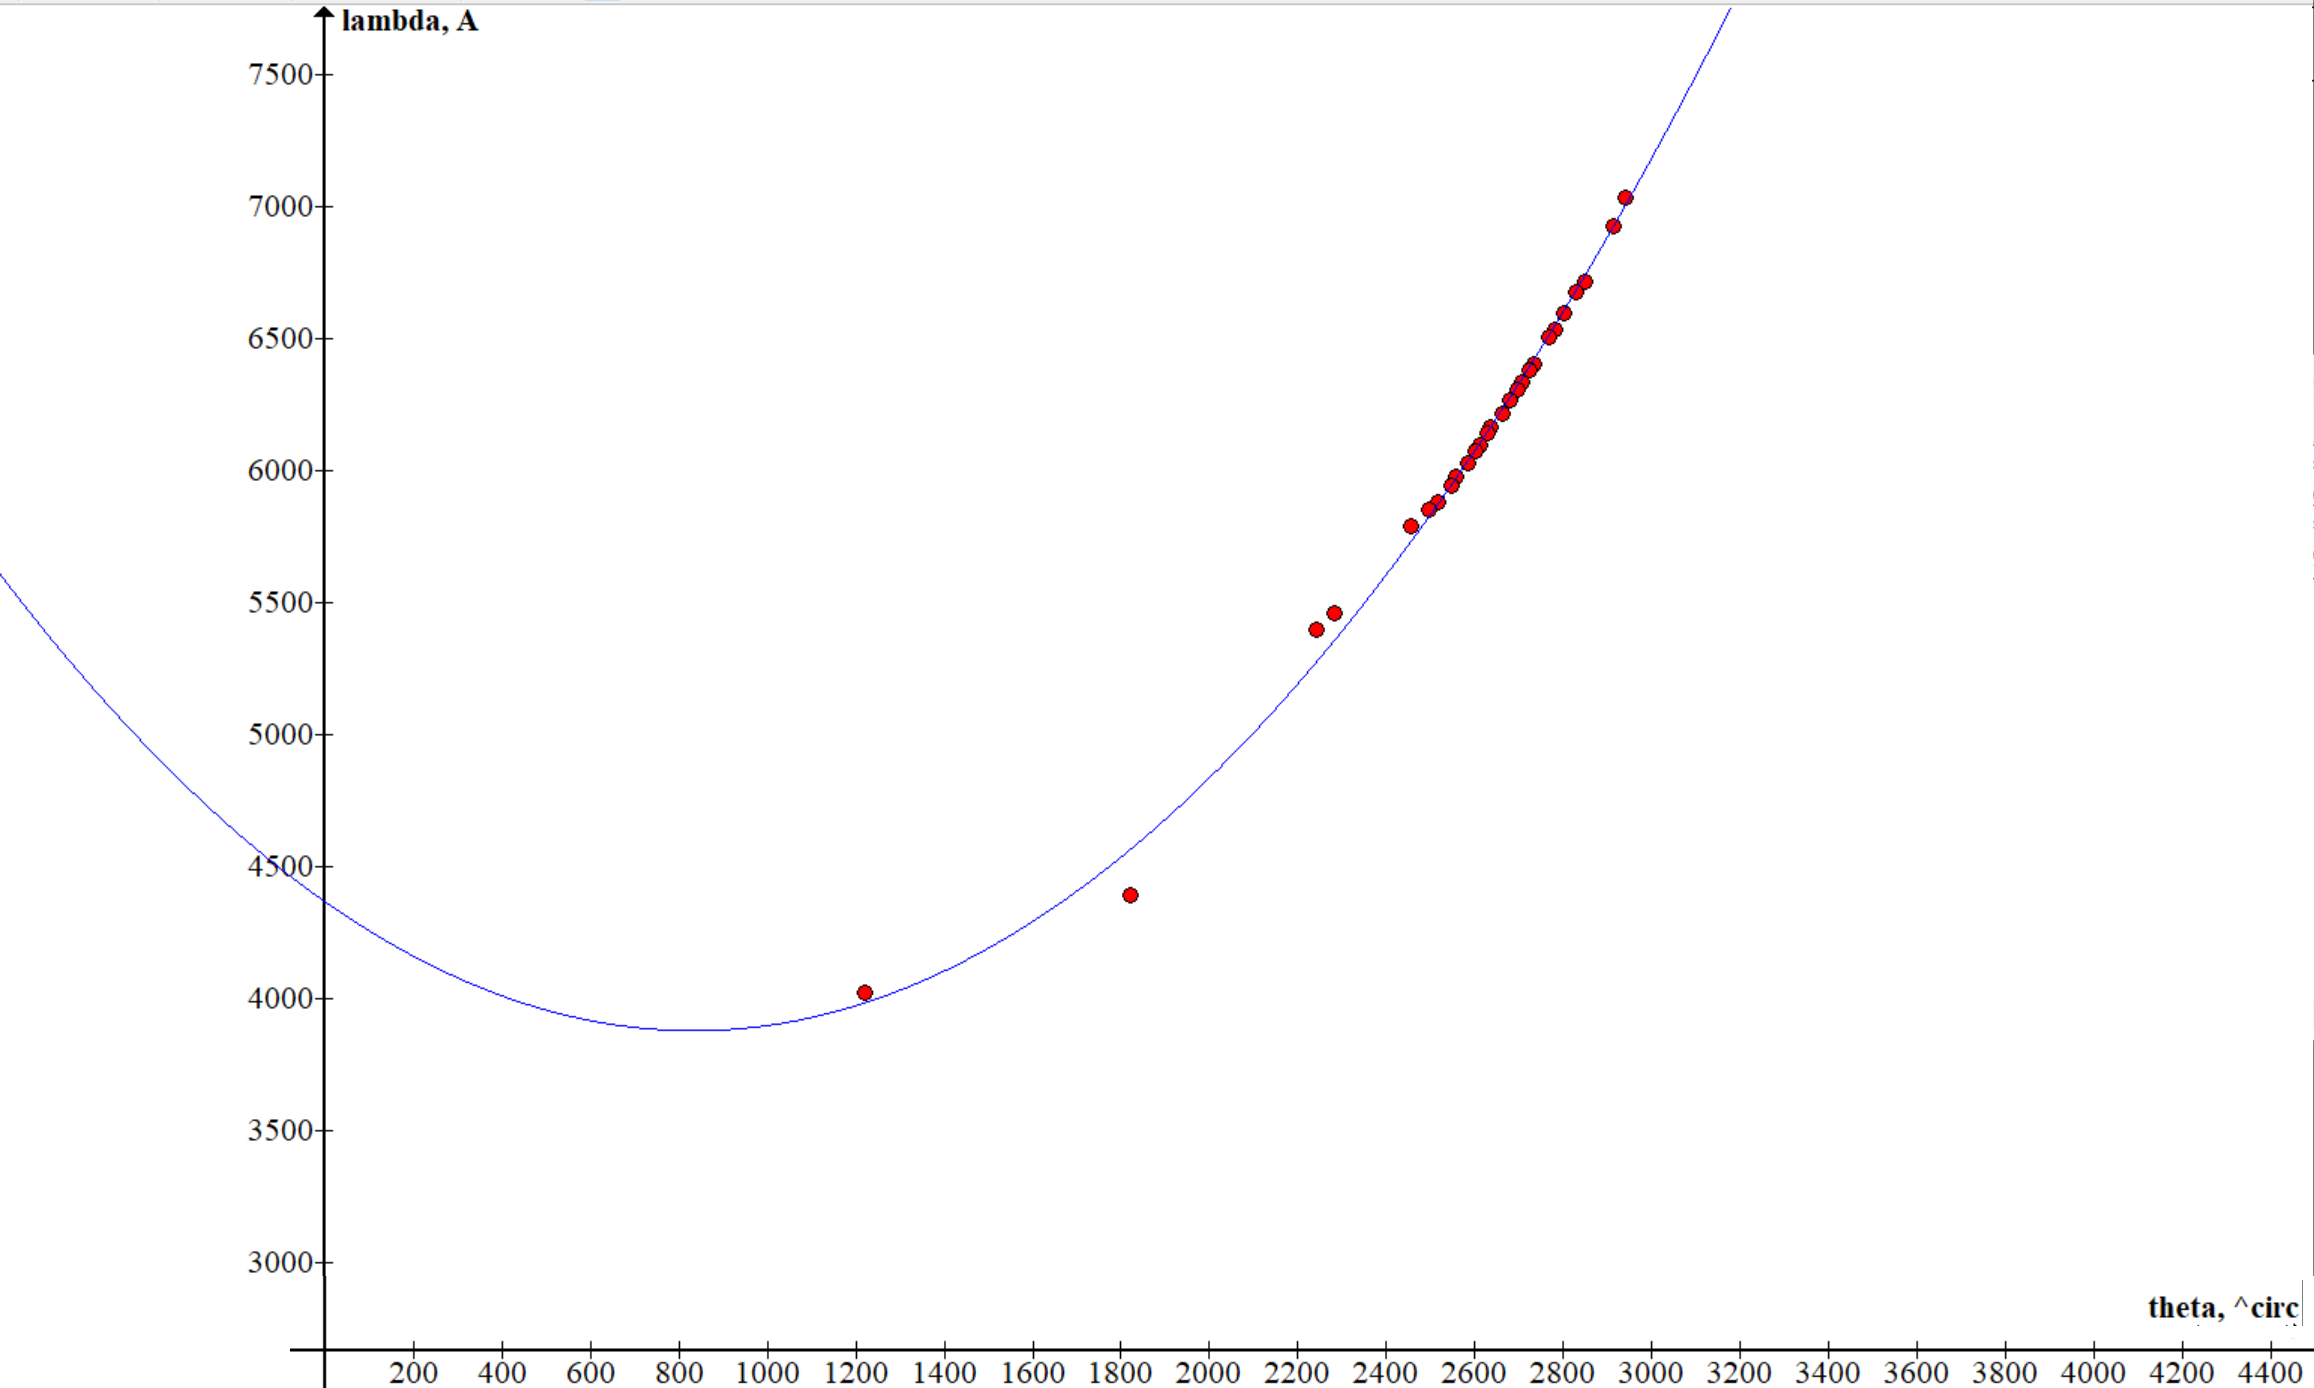
\includegraphics[width=1.0\linewidth]{grad.png}
  \caption{Градуировка спектрометра}
  \label{al}
\end{figure}

Получаем приближение полиноном второй степени:

\[ f(x) = 0,0007x^{2} -1,1725x + 4444 \]


С учётом градуировки спектрометра получаем следующие длины волн для
водорода:


\[  H_{\alpha} = (650\pm 15)\ \text{нм} \]
\[  H_{\beta} = (486\pm 20)\ \text{нм} \]
\[  H_{\gamma} = (430\pm  25)\  \text{нм} \]


Для каждой линии определим константу Ридберга по формуле (\ref{eq:Ry}),
учитывая, что $m=2$, $Z=1$, а также, что:

\newpage

\begin{itemize}
  \item для линии $H_{\alpha} \Rightarrow n=3$
  \item для линии $H_{\beta}  \Rightarrow n=4$
  \item для линии $H_{\gamma} \Rightarrow n=5$
\end{itemize}
Получаем следующие значения константы Ридберга:

\[ \text{Ry}_{\alpha}=(1.115\pm 0.04) \cdot 10^{-2} \ \text{нм}^{-1} \]
\[ \text{Ry}_{\beta} =(1.10\pm 0.05)\cdot 10^{-2} \ \text{нм}^{-1} \]
\[ \text{Ry}_{\gamma}=(1.11\pm 0.06)\cdot 10^{-2}\ \text{нм}^{-1} \]


Возьмем среднее среди полученных значений константы Ридберга и определим её
экспериментально полученное значение:

\[ \text{Ry}_E=(1.10\pm 0.05)\cdot 10^{-2} ~\text{нм}^{-1} \]

Полученное значение вполне совпадает с табличным значением в пределах
погрешности:

\[ \text{Ry}=1.097\cdot 10^{-2} \ \text{нм}^{-1} \]

Запишем показания спектрометра для следующих переходов в молекуле йода:
\begin{itemize}
  \item $\theta_{1,0}$ -- переход из первого колебательного уровня
        основного состояния в нулевой колебательный уровень возбуждённого
        состояния
  \item $\theta_{1,5}$ -- переход из первого колебательного уровня
        основного состояния в пятый колебательный уровень возбуждённого
        состояния
  \item $\theta_{g}$ -- переход из нулевого колебательного уровня
        основного состояния в область непрерывного спектра возбуждённого
        состояния
\end{itemize}

Получаем следующие данные:

\[  \theta_{1,0}=(2700\pm 5), \]
\[  \theta_{1,5}=(2620\pm 5), \]
\[  \theta_g=(2000\pm 5)  \]

откуда находим соответствующие длины волн:

\begin{equation*}
  \lambda_{1,0}=(620\pm 30) \ \text{нм}, \ \lambda_{1,5}=(610\pm 30) \ \text{нм}, \ \lambda_g=(510\pm 30)\ \text{нм}.
\end{equation*}

Определим энергию колебательного кванта возбуждённого состояния молекулы по
формуле:
\begin{equation*}
  h \nu_2=\dfrac{h\nu_{1,5}-h \nu_{0,5}}{5}.
\end{equation*}
Итого:

\[  h\nu_2=(1.0\pm 0.2)\cdot 10^{-2} \ \text{эВ} \]

Вычислим:
\begin{itemize}
  \item энергию электронного перехода $\Delta E=E_2-E_1$
  \item энергию диссоциации $D_1$ в основном состоянии
  \item энергию диссоциации $D_2$ в возбуждённом состоянии
\end{itemize}

При условии, что известны энергия колебательного кванта основного
состояния есть $h\nu_1=0,027$~эВ, энергия возбуждения, то есть энергия
перехода атома из области непрерывного спектра основного состояния в
область непрерывного спектра возбуждённого состояния, равна $E_A=0.94$
эВ.\\

\newpage

Имеем систему уравнений:

\begin{equation*}
  \begin{cases}
    D_1+E_A=h \nu_g,                                \\
    h\nu_g=D_2+\Delta E,                            \\
    h\nu_{1,0} =\Delta E+h\nu_2-\dfrac{3}{2}h\nu_1, \\
    h\nu_{1,5}=\Delta E+\dfrac{11}{2}h\nu_2-\dfrac{3}{2}h\nu_1.
  \end{cases}
\end{equation*}

Из неё находим все необходимые величины:
\[ \Delta E=(2.0\pm 0.1) \ \text{эВ} \]
\[  D_1=(1.5\pm 0.1)\  \text{эВ}  \]
\[ D_2=(0.42\pm 0.1) \ \text{эВ} \]